\chapter{解不等式}
\section{二次不等式与分式的解法}
\subsection{一元二次方程:$ax^2+bx+c=0(a \neq 0 )$}
\begin{enumerate}
	\item 解法 $x_1,x_2=\frac{-b\pm\sqrt{b^2-4ac}}{2a}$.
	\item 判别式  
	 \begin{enumerate}
		\item $\Delta >0$ ,有两个不相等的实数根.
		\item $\Delta =0$ ,有两个相等的实数根.
		\item $\Delta <0$ ,无实数根.
	\end{enumerate}
	\item 跟与系数的关系:$x_1+x_2=-\frac{b}{a}$、$x_1*x_2=\frac{c}{a}$.
	\item 根与函数的关系.
	\item 根与不等式的关系(等是不等的界).
\end{enumerate}
\subsection{二次函数:$y=ax^2+bx+c(a \neq 0 )$}

对称轴在内还是在外,在外为左还是右,内那边靠对称轴(max.min)。
\subsection{一元二次不等式}
\begin{enumerate}
	\item 一般式:$ax^2+bx+c>$或$ax^2+bx+c<0(a\neq 0)$
	\item 解法:函数法.
\end{enumerate}
\begin{figure}[h]
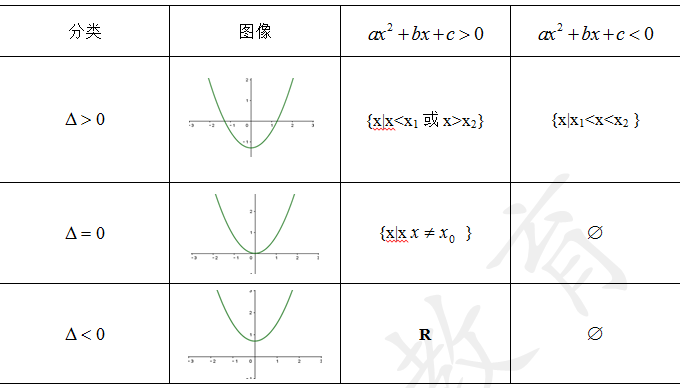
\includegraphics[scale=0.69]{1.png}
\end{figure}
\subsection{分式不等式}
\begin{enumerate}
	\item 一般式$\frac{f(x)}{g(x)}>0$或$\frac{f(x)}{g(x)}<0$.
	\item 解法:商化积$\frac{f(x)}{g(x)} >0$ $\Rightarrow f(x)g(x)>0$或$\frac{f(x)}{g(x)}<0$ $\Rightarrow f(x)g(x)<0$(穿根法).
\end{enumerate}
\section{例题分析}
\begin{example}解不等式 \par
(1).$2x^2-3x-2>0$   \hfil  (2)$-3x^2+6x>2$ \par
\vspace{2cm}
(3).$4x^2-4x+1>0$   \hfil  (4).$-x^2+2x-3>0$\\
\vspace{2cm}
\end{example}
\begin{example}解不等式\\
	(1).$(x-1)(x-a)<0$     \hfil   (2).$(x-1)(ax-1)>0$ \hfil  (3).$(x^2+6x+9)(x+1)>0$\\
	\vspace{2cm}
\end{example}
\begin{example}解不等式\\
	(1).$\dfrac{x-3}{x+7}<0$\hfil   (2).$\dfrac{1-2x}{x+4}\leq 0$ \hfil (3).$x^4-2x^2-8>0$\\
	\vspace{2cm}
\end{example}
\begin{example}解关于x的不等式$\frac{x-a}{x^2-3x-4}\leq(0\in R)$\\
	\vspace{2cm}
\end{example}
\begin{example}已知:方程$(m+1)x^2+2(2-m)x+2m+4=0(m\in R)$,求m为何值时一根大于3,一根小于3.\\
	\vspace{2cm}
\end{example}
\begin{example}解关于x的不等式\par
	(1)$x^2-2(a+1)x+1<0(a\in R)$\par
	\vspace{2cm}
	(2)$ax^2-(a-8)x+1>0(a\in R)$\par
	\vspace{2cm}
	(3)$kx^2-2(k-1)x+k+2>0(k\in R)$
	\vspace{2cm}
\end{example}
\chapter{绝对值不等式}
\section{含绝对值不等式的解法}
%%\subsection{含绝对值不等式的解法}
\begin{enumerate}
	\item 定义法:\begin{enumerate}
		\item $|x|<a(a>0)\Leftrightarrow -a<x<a$
		\item $|x|>a(a>0)\Leftrightarrow  x>a\text{或} x<-a$ 
		\item 含多个绝对值,用零点分区间.
	\end{enumerate}
	\item 公式法:\begin{enumerate}
		\item $|f(x)|<g(x)\Leftrightarrow -g(x)<f(x)<g(x)$
		\item $|f(x)|>g(x)\Leftrightarrow  f(x)>g(x)\text{或} f(x)<-g(x)$
	\end{enumerate}
\end{enumerate}
\section{例题分析}
\begin{example}解不等式\par
	(1).$|x-500|\leq 5$  \hfil   (2)$|2x+5|>7$\par
	\vspace{2cm}
	(3).$|x-a|<b$\hfil  (4).$|2x+1|+|x-2|>4$
	\vspace{2cm}
\end{example}
\begin{example}解不等式\par
	(1).$(1-|x|)(x+1)>0$  \hfil   (2)$|x^2-x-8|\geq x$\par
	\vspace{2cm}
	(3).$|\sqrt{x-2}-3|>1$\hfil  (4).$x^2-5|x|+6<0$\par
	\vspace{2cm}
	(5).$|x+7|-|3x-4|+\sqrt{3-2\sqrt{2}}>0$
	\vspace{2cm}
\end{example}
\begin{example}
	解关于x的不等式$(2x-1)a^2+(5x-2)a>3(x-1)(a\in R)$\\
	\vspace{2cm}
\end{example}
\begin{example}
   已知不等式$ax^2+bx+c>0$的解为$-3<x<1$,求不等式$cx^2+(a+b)x+6(b-a)<0$的解.
   \vspace{2cm}
\end{example}
\begin{example}解答\par
		(1).集合$\{x|0<|x-1|<3,x\in Z\}$的真子集个数.\par
		\vspace{2cm}
	(2).求使$\frac{\sqrt{3-|x|}}{\sqrt{|2x+1|-4}}$有意义的x的集合.\par
	\vspace{2cm}
	(3).已知$A=\{x||x-a|\leq 2\},B=\{x||x-1|\geq 3\}且A\cap B=\emptyset$则实数a的取值范围.\par
	\vspace{2cm}
	(4).若$a>0$,使不等式$|x-4|+|x-3|<a$的解集不是空集的a的范围.
	\vspace{2cm}
\end{example}
\begin{example}
	已知函数$f(x)=|x+1|-|x-2|$\par
	(1).求不等式$f(x)\geq 1$的解集;\par
	(2).若不等式$f(x)\geq x^2-x+m$的解集非空,求m的取值范围.\\
	\vspace{2cm}
	\end{example}
	\begin{example}
		已知$f(x)=|x+1|-|ax-1|$\par
		(1).当a=1时,求不等式$f(x)>1$的解集\par
		(2).当$x\in(0,1)$时不等式$f(x)>x$成立,求a的取值范围.
	\end{example}
	